\documentclass[12pt]{article}

\usepackage[francais]{babel}
\usepackage[utf8]{inputenc}
\usepackage[T1]{fontenc}
\usepackage{graphicx}
\usepackage[hidelinks]{hyperref}
\usepackage[left=3cm, right=3cm, top=3cm, includefoot]{geometry}
\usepackage{fancyhdr}
\pagestyle{fancy}
\fancyhead{}
\fancyfoot{}
\fancyfoot[R]{ \thepage\ }
\renewcommand{\headrulewidth}{pt}
\renewcommand{\footrulewidth}{1pt}

\newcommand{\hsp}{\hspace{20pt}}
\newcommand{\HRule}{\rule{\linewidth}{0.5mm}}

\begin{document}
\tableofcontents
\thispagestyle{empty}
\cleardoublepage

\setcounter{page}{1}
\rfoot{\textit{\textbf{Page \thepage}}}
\rhead{\textit{\textbf{Chapite 3: Conception de la solution proposée}}}
\section{Introduction}
L’enfant cancéreux souffre en silence, il affronte de sérieux problèmes. Sa maladie est mortelle, on doit s’occuper de lui et trouver des solutions pour déminuer sa souffrance.

Pour cela on utilise des outils inventé par l'Homme pour faciliter la tache de la surveillance de cet 
enfant, tel que la caméra thermique.
\section{Objectif}
Notre contribution est la réalisation du modèle basée sur l’apprentissage automatique qui détecte la température corporelle de l'enfant cancéreux, basé sur une image thermique.

Pour cela on utilise des images thermiques prisent périodiquement (la période sera définie par le professionnel de santé), la période souvent estimée à deux heures, elle fera l’objet d’entrée dans le modèle établi afin de déduire la température corporelle de l’enfant.

Si la température est élevée (cas de fièvre) une alerte se lancé par le système afin d’avertir l'infirmière ou le médecin, la présence d'un des deux n'est pas indisponsable tout le temps cela lui permet de s’occuper des autres malades qui ont vraiment besoin d’elle.
\section{Architecture générale de la solution}
\begin{figure}[h]
	\centering
	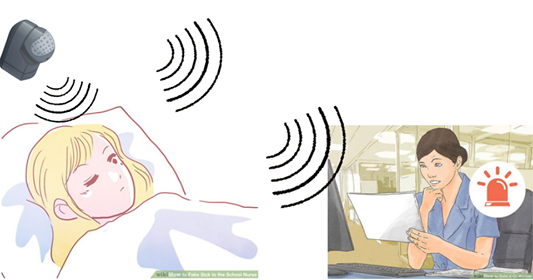
\includegraphics[height=10cm,width=15cm]{img-Chapiter-3/processus.png}
	\caption{Processus générale}
\end{figure}
\newpage
\subsection{Présentation}
Notre processus c’est une caméra thermique au-dessus d’un lit d’un malade relie avec un Raspberry Pi, cette caméra va photographier l’enfant d'un temps précis à l'autre, cette image va être transmise au modèle (il est dans le Raspberry Pi), ce dernier va la traiter, au cas de fièvre une alerte est lancée à l’infirmière au même temps cette image va être sauvegardée avec la décision et les coordonnés de l’enfant.

\subsection{Objectifs de processus générale}
\begin{itemize}
	\item Être plus civilisé qu’avant.
	\item Aider l’être humain par des appareils qui font les même fonctions que l’homme.
	\item L’enfant sera surveillé et sous contrôle tout le temps.
	\item Quant à l'infirmière le fait de surveiller le malade de temps en temps c'est très fatiguant en utilisant cette processus on gagne du temps, on fournit moins d'efforts qu'avant et en augmentant la précision.	
	\item Quand l'infirmière vient voir l'enfant d'un temps à l'autre elle le dérange mais avec cette processus il est plus à l'aise, même si l'enfant est endormi cet appareil peut prendre des photos et peut lancer des alertes sans le moindre dérangement.
\end{itemize}

\subsection{Présentation et description de chaque couche}
\begin{enumerate}
		\item La 1\textsuperscript{èr} couche: Notre dispositif sera posé sur la tête de lit de malade. 
		\item La 2\textsuperscript{ème} couche: Raspberry Pi qui contient  un modèle pour estimer la température et une base de données pour sauvegarder les données.
		\item La 3\textsuperscript{ème} couche: Interface qui détecte les alerte lancé par le système.
\end{enumerate}

\subsection{Déroulement de la processus générale}
La caméra thermique se trouve au tête de lit d'un enfant cancéreux, cette caméra est relie avec un Raspberry Pi, cette dernière photographie cet enfant de temps en temps, elle envoie la photo prise au modèle qui va la traiter et donne la décision selon la température de l'enfant, si la température est élevée une alerte sera lancée a l'infirmière ou au médecin, ils le prennent en charge, si la température est normale il y aura aucune alerte.

L'image prise, la décision et les coordonnées de l'enfant seront sauvegardées dans une base de données.
   
\section{Architecture Détaillée}
\subsection{Matériel}
\begin{itemize}
	\item \textbf{Caméra thermique} [3] qui a comme fonction la prise des images thermiques.
	%https://www.adafruit.com/product/3538
	\begin{enumerate}
	\item \textbf{Description}\\
Ajoutez de la vision thermique à votre projet et avec une discussion Grille-EYE Adafruit AMG8833! Ce capteur de Panasonic est un réseau 8x8 de capteurs thermiques infrarouges. Lorsqu'il est connecté à votre microcontrôleur (ou à framboise Pi), il renvoie un tableau de 64 lectures de température infrarouge individuelles sur I2C. C'est comme ces caméras thermiques sophistiquées, mais suffisamment compactes et simples pour une intégration facile.

Cette partie mesurera des températures allant de 0 ° C à 80 ° C avec une précision de + - 2,5 ° C (4,5 ° F). Il peut détecter un être humain à une distance maximale de 7 mètres (23 pieds). Avec une fréquence d'images maximale de 10 Hz, il est idéal pour créer votre propre détecteur humain ou mini caméra thermique. Nous avons du code pour utiliser cette connexion sur un Arduino ou compatible (le capteur communique sur I2C) ou sur un Raspberry Pi avec Python. Sur le Pi, avec un peu d'aide au traitement des images de la bibliothèque SciPy python, nous avons pu interpoler la grille 8x8 et obtenir de très bons résultats!

L'AMG8833 est la nouvelle génération de capteurs infrarouges thermiques 8x8 de Panasonic et offre des performances supérieures à celles de son prédécesseur, l'AMG8831. Le capteur prend uniquement en charge I2C et dispose d'une broche d'interruption configurable pouvant se déclencher lorsqu'un pixel individuel dépasse ou dépasse un seuil que vous avez défini.

	\item \textbf{Détails techniques}\\
	Dimensions du produit: 25.8mm x 25.5mm x 6.0mm / 1.0 "x 1.0" x 0.2 "
	
	Poids du produit: 2.9g / 0.1oz
	\item \textbf{Caractéristiques}\\
	La caractéristique qualitative principale d’une caméra infrarouge thermique peut se résumer par sa courbe MRTD \footnote{Minimum resolvable temperature difference} qui correspond à l’évolution de la résolution thermique (plus petit objet visible) en fonction de la résolution spatiale (plus petit contraste de température perceptible).
	\item \textbf{Prix}\\
	Le prix de cette caméra thermique est  \$ 39.95  
	\newpage
\end{enumerate}	 

\begin{figure}[h]
	\centering
	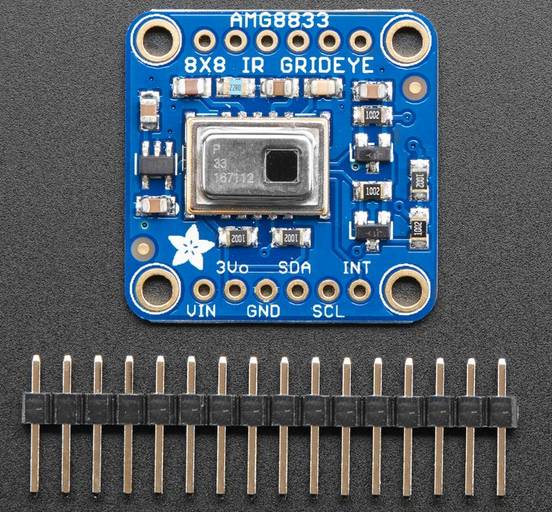
\includegraphics[height=9cm,width=12cm]{img-Chapiter-3/ther.png}
	\caption{Adafruit AMG8833 IR Thermal Camera}
\end{figure}

	\item \textbf{Raspberry Pi 2 Model B [4]}
	% https://thepihut.com/products/raspberry-pi-2-model-b?variant=18198528708
	\begin{enumerate}
		\item \textbf{Description}\\
	Le Raspberry Pi est un ordinateur au format carte de crédit. Le Raspberry Pi 2 Model B est la deuxième génération de Raspberry Pi. Il est basé sur le système sur puce (SoC) BCM2836, qui comprend un processeur ARM Cortex-A7 à quatre cœurs et un puissant processeur graphique.\\
		
		Le Raspberry Pi 2 Model B est à un niveau totalement nouveau par rapport à ses prédécesseurs en étant 6 fois plus rapide que le Raspberry Pi Model B +.
		\item \textbf{Caractéristiques}\\
		\begin{enumerate}
		\item 6 fois plus rapide - Ordinateur à carte unique alimenté par processeur Broadcom BCM2836 ARMv7 à quatre cœurs fonctionnant à 900 MHz.
		\item Double mémoire - 1 Go de RAM pour que vous puissiez maintenant exécuter des applications plus grandes et plus puissantes.
		\item Une disposition et une empreinte de carte identiques à celles du modèle B +, de sorte que tous les boîtiers et cartes complémentaires tierces conçus pour le modèle B + soient entièrement compatibles.
		\item Entièrement compatible avec HAT.
		\item GPIO étendu à 40 broches pour améliorer vos projets «réels». GPIO est 100\% compatible avec les cartes Modèle B + et A +. Les 26 premières broches sont identiques aux cartes Modèle A et Modèle B pour assurer une compatibilité ascendante complète entre toutes les cartes.
		\item Connectez une caméra Raspberry Pi et un écran tactile (vendus séparément).
		\item Diffusez et regardez une sortie vidéo haute définition en 1080P.
		\item Emplacement Micro SD pour stocker des informations et charger vos systèmes d'exploitation.
		\item Gestion de l'alimentation avancée:
		
		\begin{enumerate}
			\item Vous pouvez désormais fournir jusqu'à 1,2 A aux ports USB, ce qui vous permet de connecter davantage de périphériques USB gourmands en énergie directement au Raspberry PI. (Cette fonctionnalité nécessite une alimentation micro USB 2Amp)
		\end{enumerate}
		\item Port Ethernet 10/100 pour connecter rapidement le Raspberry Pi à Internet.
		\item Prise combinée à 4 pôles pour connecter votre sortie audio stéréo et votre sortie vidéo composite.
\end{enumerate}
	\item \textbf{Spécifications techniques}\\
		\begin{enumerate}
			\item Ordinateur à carte unique alimenté par processeur Broadcom BCM2836 ARMv7 à quatre cœurs fonctionnant à 900 MHz.
			\item 1 Go de RAM.
			\item GPIO étendu à 40 broches.
			\item 4 x ports USB.
			\item Sortie stéréo 4 pôles et port vidéo composite.
			\item HDMI pleine taille.
			\item Port de caméra CSI pour connecter la caméra Raspberry Pi.
			\item Port d’affichage DSI pour connecter l’écran tactile Raspberry Pi.
			\item Port Micro SD pour le chargement de votre système d'exploitation et le stockage de données.
			\item Source d'alimentation micro USB.
\end{enumerate}
\newpage
	\item \textbf{Prix}\\
	Le prix de Raspberry Pi 2 Model B est \$ 43.32
	\end{enumerate}
	\begin{figure}[h]
		\centernig
		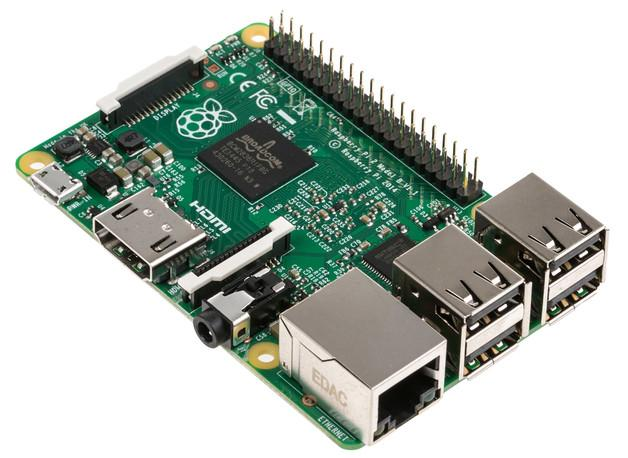
\includegraphics[height=10cm,width=12cm]{img-Chapiter-3/raspbPi.jpg}
		\caption{Raspberry Pi 2 Model B}
	\end{figure}\\
	
	
	Un prototype d'une caméra thermique \textit{Adafruit AMG8833 IR} relie avec un Raspberry Pi 
	\begin{figure}[h]
				\centering
		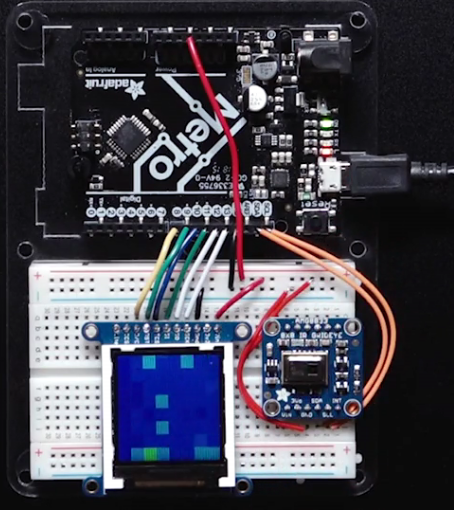
\includegraphics[height=10cm,width=12cm]{img-Chapiter-3/therPi.png}
		\caption{caméra thermique \textit{Adafruit AMG8833 IR} relie avec un Raspberry Pi }
	\end{figure}
\end{itemize}
\newpage



\subsection{Principe de fonctionnement}
\begin{itemize}
	\item \textbf{Étape 1}\\
	Une caméra thermique qui prend l'image de visage de l'enfant, l'enfant doit être juste sous la caméra dont la distance est de 2 mètres, pour qu’elle puisse prendre une image claire de son visage, cette caméra est reliée avec un Raspberry Pi.
	\item \textbf{Étape 2}\\
	Quand la caméra thermique prend le visage de l'enfant, l'image sera envoyée  au modèle qui va traiter l'image de l’enfant et estime la température.\\
	L'image, la décision, et les coordonnées de l'enfant serons sauvegardées dans une base de données.
	\item \textbf{Étape 3}\\
	En cas la température est élevée notre système lance une alerte.\\
	Cette alerte sera détectée par l'interface chez l'infirmière. 
\end{itemize}
\newpage

\begin{figure}[h]
	\centering
	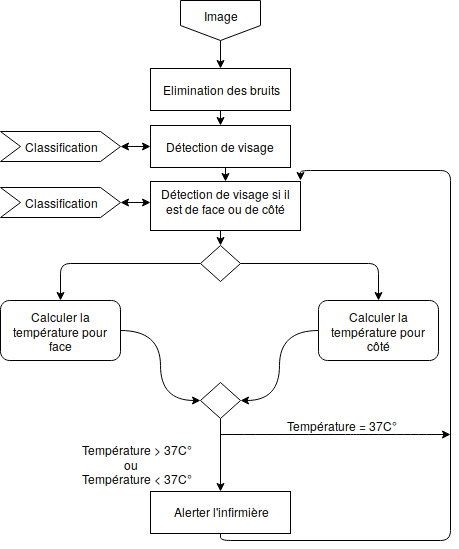
\includegraphics[height=12cm,width=12cm]{img-Chapiter-3/Picture1.png}
	\caption{Plan de travail}
\end{figure}

\section{\' Etapes de la solution}
Notre plan de travail se base sur quelques étapes:
\begin{enumerate}
	\item Faire entrer l’image thermique de l’enfant.
	\item \' Elimination des bruits trouvés dans cette image, on utilise des algorithmes tels que Papper and salt, Gaussian Blur on utilise kernel $3 \times 3$, 
	\item Détection de visage de l’enfant ça sert à classifier l’image prise, pour classifier cette image on utilise le \textit{haar cascade}.
	\item Détection s’il s’agit  de face ou de côté ça sert à classifier l’image.
	\item Calcule de la température pour visage et coté. 
	\item si la température est élevée:
	\begin{enumerate}
		\item une alerte est lancée à l’infirmière,
		\item l'image, décision et les coordonnées serons sauvegardées dans une base de données. 
		\item l’opération se répète à partir de  l’étape 4.
	\end{enumerate}
	\item si la température est normale:
	\begin{enumerate}
		\item l'image, décision et les coordonnées serons sauvegardées dans une base de données.
		\item l’opération se fait à nouveau à partir de l'étape 4.
	\end{enumerate}
\end{enumerate}

\subsection*{Gaussian Blur}
\subsubsection*{Définition}
Gaussian Blur (également appelé lissage gaussien) résulte du flou d'une image par une fonction gaussienne. C'est un effet largement utilisé dans les logiciels graphiques, généralement pour réduire le bruit de l'image et les détails. L’effet visuel de cette technique de flou est un flou lisse ressemblant à celui de la visualisation de l’image à travers un écran translucide, produit par un objectif flou ou l’ombre d’un objet sous un éclairage habituel. Le lissage gaussien est également utilisé comme étape de prétraitement dans les algorithmes de vision par ordinateur afin d'améliorer les structures d'images à différentes échelles.
\subsection*{Haar Cascade}
\subsubsection*{Définition}
Haar Cascade est fondamentalement un classificateur utilisé pour détecter l'objet pour lequel il a été formé, à partir de la source.

La Haar Cascade est formée en superposant l'image positive sur un ensemble d'images négatives. La formation se fait généralement sur un serveur et à différentes étapes. De meilleurs résultats sont obtenus en utilisant des images de haute qualité et en augmentant le nombre d'étapes pour lesquelles le classificateur est formé.

On peut également utiliser des cascades Haar prédéfinies, disponibles sur [16]
%https://github.com/opencv/opencv/tree/master/data/haarcascades

Voici une capture présente comment détecter le visage d'un enfant à partir d'une image thermique avec l'utilisation de haar cascade.
\newpage
\begin{figure}[h]
	\centering
	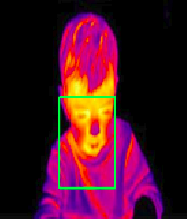
\includegraphics[scale=1]{img-Chapiter-3/enfant.png}
	\caption{Détection de visage avec Haar cascade}
\end{figure}
\section{Conclusion}
Les enfants cancéreux doivent être surveillés tout le temps, le processus dont on a parlé facilite cette tâche d’une manière plus rapide et plus sure. 
\end{document}
